\documentclass[12pt]{article}
\usepackage{graphicx}
\usepackage{enumitem}
\usepackage{multicol}
\usepackage{mathtools}
\usepackage{hyperref}
\usepackage[margin=1in]{geometry}
\usepackage{amsmath,amsthm,amssymb}

 
\begin{document}
 
% --------------------------------------------------------------
%                         Start here
% --------------------------------------------------------------
 
\title{AST1430 Assignment 3}
\author{Jessica Campbell}
\date{March 13, 2018}
\maketitle

Perhaps if the days were substantially longer I may have been able to complete this assignment.

% --------------------------------------------------------------
%               1. Emission of Ly-a from an HII Region
% --------------------------------------------------------------

\section{Emission of Ly$\alpha$ from an $\mathrm{HII}$ Region}

This involves a lot of order-of-magnitude estimates.

% --------------------------------------------------------------
%               Part 1)
% --------------------------------------------------------------

\subsection*{Part 1}

Estimate the neutral fraction for hydrogen in an $\mathrm{HII}$ region around an O6 star. The Stromgren sphere has a radius $r_s \sim 100\,\mathrm{pc}$ and a mean density of $1/\mathrm{cm^3}$. Note that an ionizing photon (Ly-continuum) has a mean-free-path of order the Stromgren radius.

% --------------------------------------------------------------
%               Solution
% --------------------------------------------------------------

\subsection*{Solution}

Since we know that the mean-free-path is given by

\begin{align*}
\ell_\mathrm{mfp} = \frac{1}{n\sigma_\nu}
\end{align*}

where $n$ is the number density and $\sigma_\nu$ is the cross section, we can solve for the number density via

\begin{align*}
n = \frac{1}{\ell_\mathrm{mfp}\sigma_\nu}.
\end{align*}

We're given that the mean-free-path is of order the Stromgren radius so $\ell_\mathrm{mfp} = 100\,\mathrm{pc}$ and the ionization cross-section is given by

\begin{align*}
\sigma_\nu = 6\times10^{-18}\left(\frac{\nu}{\nu_0}\right)^3\,\mathrm{cm^2}.
\end{align*}

Assuming $\nu=\nu_0$ corresponds to the ionization frequency of hydrogen at $13.6\,\mathrm{eV}$, the ionization cross section simplifies to $\sigma_\nu = 6\times10^{-18}$.

The ionization fraction of hydrogen $X$ is then found via:

\begin{align*}
X = \frac{n_\mathrm{HI}}{n_\mathrm{H}} \\
X = \left(\frac{1}{\ell_\mathrm{mfp}\sigma_\nu}\right) \left(\frac{1}{n_\mathrm{H}}\right) \\
X = \frac{1}{(100\,\mathrm{pc})(6\times10^{-18}\,\mathrm{cm^2})(1\,\mathrm{cm^{-3}})} \\
X = 0.0054
\end{align*}

The neutral hydrogen fraction is therefore only

\begin{align*}
\boxed{ X = 0.54\% },
\end{align*}

meaning that $99.46\%$ of the hydrogen atoms in the $\mathrm{HII}$ region are ionized.

% --------------------------------------------------------------
%               Part 2)
% --------------------------------------------------------------

\subsection*{Part 2}

What is the mean-free-path for a Ly$\alpha$ photon ($n=2 \leftarrow \rightarrow n=1$) in the same environment? The Einstein coefficient $A_{\mathrm{Ly}\alpha} \approx 6\times10^{8}\,\mathrm{s^{-1}}$.

% --------------------------------------------------------------
%               Solution
% --------------------------------------------------------------

\subsection*{Solution}

Recalling that the mean-free-path is expressed in terms ofthe absorption coefficient $\alpha_\nu$ via,

\begin{align*}
\ell_\mathrm{mfp} = \frac{1}{\alpha_\nu},
\end{align*}

we can used the expression for the absorption coefficient that we derived in the first assignment:

\begin{align}
\alpha = \frac{c^2}{8\pi\nu^2}n_aA_{21}\frac{g1}{g2}\left[ 1 - \mathrm{exp}\left(-\frac{{\Delta}E}{k_BT}\right)\right]\phi(\nu).
\end{align}

Also recall that for Doppler-broadened line profiles,

\begin{align*}
\phi(\nu) = \frac{1}{\sqrt{\pi}\Delta\nu_D}\mathrm{exp}\left[-\left(\frac{\nu - \nu_0}{\Delta\nu_D}\right)^2\right],
\end{align*}

where $\Delta\nu_D$ is the line width and is related to the Doppler parameter $b$ (matter sound speed) as $\Delta\nu_D \approx (b/c)\nu_0$. So the absorption coefficient can be written as:

\begin{align}
\alpha = \frac{c^2}{8\pi\nu^2}n_aA_{21}\frac{g1}{g2}\left[ 1 - \mathrm{exp}\left(-\frac{{\Delta}E}{k_BT}\right)\right] \frac{1}{\sqrt{\pi}\Delta\nu_D}\mathrm{exp}\left[-\left(\frac{\nu - \nu_0}{\Delta\nu_D}\right)^2\right].
\end{align}

Since we are assuming $\nu=\nu_0$, this simplifies to

\begin{align}
\alpha = \frac{c^2}{8\pi\nu^2}n_aA_{21}\frac{g1}{g2}\left[ 1 - \mathrm{exp}\left(-\frac{{\Delta}E}{k_BT}\right)\right] \frac{1}{\sqrt{\pi}\Delta\nu_D}.
\end{align}

If we assume that the matter sound speed is $0.1c$, $\Delta\nu_D \approx 0.1\nu_0$ which allows us to write the absorption coefficient as:

\begin{align}
\alpha = \frac{c^2}{8\pi\nu^2}n_aA_{21}\frac{g1}{g2}\left[ 1 - \mathrm{exp}\left(-\frac{{\Delta}E}{k_BT}\right)\right] \frac{1}{\sqrt{\pi}0.1\nu_0}.
\end{align}

% --------------------------------------------------------------
%               Part 3)
% --------------------------------------------------------------

\subsection*{Part 3}

A Ly$\alpha$ photon can also freely escape the $\mathrm{HII}$ region if it gets absorbed by a (very) fast moving stom and gets re-emitted at a frequency that is optically thin. Assuming the line profile is thermally broadened with a temperature $T \sim 10^4\,\mathrm{K}$ (typical of an $\mathrm{HII}$ region), how far away from the line centre does the new frequency have to be? Compared with diffusion by random walk (see above) through the $\mathrm{HII}$ region, is this process more likely?

% --------------------------------------------------------------
%               Solution
% --------------------------------------------------------------

\subsection*{Solution}



% --------------------------------------------------------------
%               Part 4)
% --------------------------------------------------------------

\subsection*{Part 4}

What is the fraction of neutral hydrogen that is in the $n=2$ state? To answer this question, we split it into two parts. Ionized hydrogen can recombime, with roughly similar probabilities, into the $2s$ and $2p$ state. This part looks at the $2s$ state. The transition between $2s$ and $1s$ is forbidden by dipole selection rules. However, an exotic process called the 2-photon process can happen and produces a transition probability of $A_{2\gamma} = 8.23\,\mathrm{s^{-1}}$. Argue that for our $\mathrm{HII}$ region, this latter process dominates over collisional process in depopulating the $2s$ state. Table 3.12 of Osterbrock gives the collision strength between electron and H-atoms, $\Omega\approx0.26$. Obtain the fraction of neutral hydrogen in the $2s$ state.

% --------------------------------------------------------------
%               Solution
% --------------------------------------------------------------

\subsection*{Solution}



% --------------------------------------------------------------
%               Part 5)
% --------------------------------------------------------------

\subsection*{Part 5}

On the other hand, the transition between $2p$ and $n=1$ is allowed. Estimate which of the following rates aree important for the $2p$ state: radiative recombination (+); electron collisional excitation from the $n=1$ and $2s$ states ($+$); radiative pumping by Ly$\alpha$ photons ($+$); spontaneous emission to the $n=1$ stzte ($-$); spontaneous emission to the $2s$ state ($-$); electron collisional deexcitation to the $n=1$ and $2s$ states ($-$). Take the relative numbers of Ly$\alpha$ and Ly-continuum photons to be their relative residence times in the $\mathrm{HII}$ region. What is the fraction of neutral hydrogen in the $2p$ state?

% --------------------------------------------------------------
%               Solution
% --------------------------------------------------------------

\subsection*{Solution}



% --------------------------------------------------------------
%               Part 6)
% --------------------------------------------------------------

\subsection*{Part 6}

Estimate the Einstein coefficient for a Balmer-$\alpha$ photon ($n=2 \leftarrow\rightarrow n=3$), and compare your result with what you obtain by querying the NIST database. What is the integrated optical depth at its line centre?

% --------------------------------------------------------------
%               Solution
% --------------------------------------------------------------

\subsection*{Solution}



% --------------------------------------------------------------
%               Part 7)
% --------------------------------------------------------------

\subsection*{Part 7}

Compare the 2-photon process to those in sub-questiom 3, which one is a more likely fate for a Ly$\alpha$ photon? Relatedly, what do you think will be the dominant hydrogen lines from an $\mathrm{HII}$ region?

% --------------------------------------------------------------
%               Solution
% --------------------------------------------------------------

\subsection*{Solution}





% --------------------------------------------------------------
%                    2. Largest Atom in Space
% --------------------------------------------------------------

\section{Largest Atom in Space }


% --------------------------------------------------------------
%               Part 1)
% --------------------------------------------------------------

\subsection*{Part 1}

Using L-S coupling, determine the spectroscopic terms for the ground configuration ($2s^22p^2$) and excited configurations ($2s^22p3p, 2s^22p3s$). Mark also possible $J$ values. Which one is the ground state?

% --------------------------------------------------------------
%               Solution
% --------------------------------------------------------------

\subsection*{Solution}

\subsection*{Ground configuration ($2s^22p^2$)}

For the ground configuration ($2s^22p^2$), $2s^2$ is a filled sub-shell and it therefore does not contribute to the angular momentum so we need only determine the spectroscopic terms for the paired electrons in the $2p$ orbital. First, we calculate the total number of possible microstates via

\begin{align*}
N = \frac{t!}{e!(t-e)!},
\end{align*}

where $t = 2(2\ell+1)$ and $e$ is the number of available electrons. Since we have two paired electrons in the $2p$ orbital, $\ell=1$, $t=6$, and $e=2$:

\begin{align*}
N = \frac{6!}{2!4!} = \frac{4!\cdot5\cdot6}{2!4!} = \frac{5\cdot6}{2!} = 5\cdot3 = 15.
\end{align*}

We draw out each of these 15 possible microstates (see Table \ref{table:config1_table1}).

\begin{table}[ht]
\centering
\caption{All possible electron configurations for the ($2s^22p^2$) ground state.}
\label{table:config1_table1}
\begin{tabular}{|l|lll|ll|}
\hline 
 & \multicolumn{3}{c}{$m_\ell$} & \multicolumn{2}{|c|}{} \\
microstate & +1 & 0 & -1 & $M_L$ & $M_S$ \\
\hline
1  & $\uparrow$               & $\uparrow$              &                         & +1 & +1 \\
2  &                          & $\uparrow$              & $\uparrow$              & -1 & +1 \\
3  & $\uparrow$               &                         & $\uparrow$              &  0 & +1 \\
\hline
4  & $\downarrow$             & $\downarrow$            &                         & +1 & -1 \\
5  &                          & $\downarrow$            & $\downarrow$            & -1 & -1 \\
6  & $\downarrow$             &                         & $\downarrow$            &  0 & -1 \\
\hline
7  & $\uparrow$ $\downarrow$  &                         &                         & +2 &  0 \\
8  & $\uparrow$               & $\downarrow$            &                         & +1 &  0 \\
9  & $\uparrow$               &                         & $\downarrow$            &  0 &  0 \\
10 &                          & $\uparrow$ $\downarrow$ &                         &  0 &  0 \\
11 &                          & $\uparrow$              & $\downarrow$            & -1 &  0 \\
12 & $\downarrow$             & $\uparrow$              &                         & +1 &  0 \\
13 &                          &                         & $\uparrow$ $\downarrow$ & -2 &  0 \\
14 & $\downarrow$             &                         & $\uparrow$              &  0 &  0 \\
15 &                          & $\downarrow$            & $\uparrow$              & -1 &  0 \\
\hline
\end{tabular}
\end{table}

We can create a smaller table with each $M_L$ and $M_S$ and count up the number of such configurations (see Table \ref{table:config1_table2}) noting that $M_L \equiv \sum m_\ell$ and $M_S \equiv \sum m_s$ for $L-S$ coupling.

\begin{table}[ht]
\centering
\caption{All possible spin and angular momentum quantum number configurations for the ($2s^22p^2$) ground state.}
\label{table:config1_table2}
\begin{tabular}{|ll|lll|}
\hline
\multicolumn{2}{|c}{} & \multicolumn{3}{|c|}{$M_S$} \\
\multicolumn{2}{|c|}{} & +1 & 0 & -1 \\
\hline
      & +2 & 0 & 1 & 0 \\
      & +1 & 1 & 2 & 1 \\
$M_L$ &  0 & 1 & 3 & 1  \\
      & -1 & 1 & 2 & 1 \\
      & -2 & 0 & 1 & 0 \\
\hline
\end{tabular}
\end{table}

The maximum spin and angular momenta in these configurations are $M_S = 1$ and $M_L = 1$ respectively, so $S=1$ and $L=1$. With $L-S$ coupling, the spectroscopic terms for each configuration is given by

\begin{align*}
^(2S+1)L_J
\end{align*}

where $S$ is the total spin angular momentum, $(2S+1)$ is the spin multiplicity, $L$ is the total orbital angular momentum which defines the orbital shape, and $J$ is the total angular momentum with coupling between $L$ and $S$. Since $^{(2S+1)}L$, this provides us with the $^3P$ configuration. To find the possible $J$ values, we know that 

\begin{align*}
|L-S| \leq J \leq |L+S|,
\end{align*}

where each value increases in integer increments. This gives us total angular momenta values of

\begin{align*}
|1-1| \leq J \leq |1+1| \\
0 \leq J \leq 2 \\
J = 0,1,2.
\end{align*}

Applying this to the $^3P$ configuration, we have the spectroscopic terms $3^3P_0$, $3^3P_1$ and $3^3P_2$.

We now remove these configurations from Table \ref{table:config1_table2} which results in Table \ref{table:config1_table3}.

\begin{table}[ht]
\centering
\caption{Secondary spin and angular momentum quantum number configurations for the ($2s^22p^2$) ground state.}
\label{table:config1_table3}
\begin{tabular}{|ll|lll|}
\hline
\multicolumn{2}{|c}{} & \multicolumn{3}{|c|}{$M_S$} \\
\multicolumn{2}{|c|}{} & +1 & 0 & -1 \\
\hline
      & +2 & 0 & 1 & 0 \\
      & +1 & 0 & 1 & 0 \\
$M_L$ &  0 & 0 & 2 & 0 \\
      & -1 & 0 & 1 & 0 \\
      & -2 & 0 & 1 & 0 \\
\hline
\end{tabular}
\end{table}

Repeating the last step, the maximum spin and angular momenta in these configurations are $M_S = 0$ and $M_L = 2$ respectively, so $S=0$ and $L=2$. Since the spin multiplicity is $^{(2S+1)}L$, this provides us with the $^1D$ configuration. To find the possible $J$ values,

\begin{align*}
|L-S| \leq J \leq |L+S|
|2-0| \leq J \leq |2+0|
2 \leq J \leq 2
J = 2.
\end{align*}

Applying this to the $^1D$ configuration, we have the spectroscopic term $^1D_2$.

Repeating this step one last time, we obtain the last set of possible electron configurations in Table \ref{table:config1_table4}.

\begin{table}[ht]
\centering
\caption{Secondary spin and angular momentum quantum number configurations for the ($2s^22p^2$) ground state.}
\label{table:config1_table4}
\begin{tabular}{|ll|lll|}
\hline
\multicolumn{2}{|c}{} & \multicolumn{3}{|c|}{$M_S$} \\
\multicolumn{2}{|c|}{} & +1 & 0 & -1 \\
\hline
      & +2 & 0 & 0 & 0 \\
      & +1 & 0 & 0 & 0 \\
$M_L$ &  0 & 0 & 1 & 0 \\
      & -1 & 0 & 0 & 0 \\
      & -2 & 0 & 0 & 0 \\
\hline
\end{tabular}
\end{table}

The maximum spin and orbital angular momenta are $M_S=0$ and $M_L=0$ implying that $S=0$ and $L=0$, respectively. Obtaining the possible $J$ values, 

\begin{align*}
|L-S| \leq J \leq |L+S| \\
|0-0| \leq J \leq |0+0| \\
0 \leq J \leq 0 \\
J = 0.
\end{align*}

Thus, the final spectroscopic term is $^1S_0$.

To recap, all of the spectroscopic terms are: $3^3P_0$, $3^3P_1$, $3^3P_2$, $^1D_2$ and $^1S_0$.

To find the ground state, we can use Hund's Rules which say that:

1. The term with maximum spin multiplicity $(2S+1)$ has the lowest energy.

2. For a given multiplicity $(2S+1)$, the term with the largest value of the total orbital angular momentum $L$ has the lowest energy.

3. For a given term, in an atom with outermost sub-shell half-filled or less, the level with the lowest value of the total angular momentum quantum number $J = L+S$ lies lowest in energy. If the outermost shell is more than half-filled, the level with the highest value of $J$ is lowest in energy.

Following these rules, the terms with the greatest spin multiplicity are $^3P_0$, $^3P_1$ and $^3P_2$. Since they all have the same orbital angular momentum $L=0$, we only need to find the term that satisfies the third of Hund's rules. Since each of these sub-shells only have 1 electron with a maximum electron occupancy of 6, they are all less than half filled so the term with the largest $J$ has the lowest energy. The term $^3P_0$ is therefore the ground state.

\subsection*{Excited configuration $(2s^22p3p)$}

In contrast with the previous ground configuration, this excited configuration does not have any paired electrons since there is one electron in the $2p$ sub-shell and another in the $3p$ sub-shells (the $2s$ sub-shell is full with two electrons so we can ignore it since it does not contribute to the angular momentum). We therefore do not need to go through the entire procedure as before to ensure the Pauli-exclusion principle is obeyed. Instead, we can simply use characteristics of $L-S$ coupling to determine the spectroscopic terms. 

The possible spin angular momentum values can be determined via

\begin{align*}
|s_1 - s_2| \leq S \leq |s_1 + s_2|,
\end{align*}

where $s_1$ and $s_2$ are the spin values for the electrons in each sub-shells which gives us:

\begin{align*}
|1/2 - 1/2| \leq S \leq |1/2 + 1/2| \\
0 \leq S \leq 1 \\
S = 0, 1.
\end{align*}

We can also determine the possible orbital angular momentum values via

\begin{align*}
|\ell_1 - \ell_2| \leq L \leq |\ell_1 + \ell_2|,
\end{align*}

where $\ell_1$ and $\ell_2$ are the orbital values for the electrons in each sub-shell which gives us:

\begin{align*}
|1 - 1| \leq L \leq |1 + 1| \\
0 \leq L \leq 2 \\
L = 0, 1, 2.
\end{align*}

Putting all of these together to determine the possible total angular momentum values $J$ and their corresponding spectroscopic terms, we obtain Table \ref{table:config2_table1}.

\begin{table}[ht]
\centering
\caption{All possible configurations for the excited state $(2s^22p3p)$.}
\label{table:config2_table1}
\begin{tabular}{|c|cccc|c|}
\hline
microstate & S & L & J & (2S+1) & spectroscopic terms \\
\hline
1 & 0 & 0 & 0     & 1 & $^1S_0$ \\
2 & 0 & 1 & 1     & 1 & $^1P_1$ \\
3 & 0 & 2 & 2     & 1 & $^1D_2$ \\
4 & 1 & 0 & 1     & 3 & $^3S_1$ \\
5 & 1 & 1 & 0,1,2 & 3 & $^3P_0$, $^3P_1$, $^3P_2$ \\
6 & 1 & 2 & 1,2,3 & 3 & $^3D_1$, $^3D_2$, $^3D_3$ \\
\hline
\end{tabular}
\end{table}

\subsection*{Excited configuration $(2s^22p3s)$}

The possible spin angular momentum values can be determined are

\begin{align*}
|s_1 - s_2| \leq S \leq |s_1 + s_2| \\
|1/2 - 1/2| \leq S \leq |1/2 + 1/2| \\
0 \leq S \leq 1 \\
S = 0, 1.
\end{align*}

The possible orbital angular momentum values are

\begin{align*}
|\ell_1 - \ell_2| \leq L \leq |\ell_1 + \ell_2| \\
|1 - 0| \leq L \leq |1 + 0| \\
1 \leq L \leq 1 \\
L = 1.
\end{align*}

Putting these together to determine the possible total angular momentum values $J$ and their corresponding spectroscopic terms, we obtain Table \ref{table:config3_table1}.

\begin{table}[ht]
\centering
\caption{All possible configurations for the excited state $(2s^22p3s)$.}
\label{table:config3_table1}
\begin{tabular}{|c|cccc|c|}
\hline
microstate & S & L & J & (2S+1) & spectroscopic terms \\
\hline
1 & 0 & 1 & 1      & 1 & $^1P_1$ \\
2 & 1 & 1 & 0,1,2  & 3 & $^3P_0$, $^3P_1$, $^3P_2$ \\

\hline
\end{tabular}
\end{table}

% --------------------------------------------------------------
%               Part 2)
% --------------------------------------------------------------

\subsection*{Part 2}

A claim of the "largest atom in space" was reported by Stepkin et al. (2007, MNRAS, 374, 852). The authors detected $\mathrm{CI}$ absorption (jumping from, e.g., $n=1009$ to $n=1013$ state). Estimate the size of such an atom (e.g., $2s^22p1009p$), the orbital period for the outer electron, and the transition frequency.

% --------------------------------------------------------------
%               Solution
% --------------------------------------------------------------

\subsection*{Solution}

The configuration of this atom is such that the outer electron is at an energy level of $n=1009$. At such a high energy level (i.e., orbital radius), we can approximate the atom as a hydrogen atom allowing us to determine its size using a simple hydrogen model. Setting the Coulomb force equal to the centripetal force of the orbiting electron,

\begin{align*}
F_\mathrm{Coul} = F_\mathrm{cent} \\
\frac{k_ee^2}{r^2} = \frac{m_ev_e^2}{r},
\end{align*}

where $k_e$ is Coulomb's constant, $e$ is the charge of the electron, $m_e$ is the electron mass, $v$ is the orbital speed and $r$ is the orbital radius. Noting that the electron angular momentum is given by 
 
\begin{align*}
L = n\hbar = m_ev_er_e
\end{align*}

allows us to substitute

\begin{align*}
v_e = \left( \frac{n\hbar}{m_er_e} \right)
\end{align*}

for the electron's orbital speed. Making this substitution,

\begin{equation*}
\begin{split}
\frac{k_ee^2}{r_e} &= m_ev_e^2 \\
\frac{k_ee^2}{r_e} &= m_e \left(\frac{n\hbar}{m_er_e}\right)^2 \\
\frac{k_ee^2}{r_e} &= \frac{m_en^2\hbar^2}{m_e^2r_e^2} \\
k_ee^2 &= \frac{n^2\hbar^2}{m_er_e} \\
r_e &= \frac{n^2\hbar^2}{k_ee^2m_e} \\
r_e &= \left(\frac{\hbar^2}{k_ee^2m_e}\right) n^2
\end{split}
\end{equation*}

Noting that the term in parentheses is the Bohr radius $a_0$, this allows us to write the electron orbital radius in terms of the hydrogen Bohr radius:

\begin{align*}
r_e = a_on^2
\end{align*}

This gives us an orbital size of

\begin{align*}
\boxed{ r_e = 0.054\,\mathrm{mm} },
\end{align*}

where we have used $a_0 = 5.292\times10^{-11}\,\mathrm{m}$ for the Bohr radius.

The electron's orbital period of a circular orbit is given by

\begin{equation*}
\begin{split}
T_e = \frac{2\pi r_e}{v_e} \\
T_e = \frac{2\pi r_e}{\left( \frac{n\hbar}{m_er_e} \right)} \\
T_e = 2\pi r_e \left( \frac{m_er_e}{n\hbar} \right) \\
T_e = \frac{2\pi m_er_e^2}{n\hbar} \\
T_e = \frac{2\pi (9.11\times10^{-31}\,\mathrm{kg})(0.054\,\mathrm{mm})^2}{1009\hbar}.
\end{split}
\end{equation*}

This gives us an orbital period of

\begin{align*}
\boxed{ T_e = 1.6\times10^{-7}\,\mathrm{s^{-1}} }.
\end{align*}

To find the transition frequency, we can use the Rydberg formula for hydrogen:

\begin{equation*}
\begin{split}
\frac{1}{\lambda} = RZ \left( \frac{1}{n_1^2} - \frac{1}{n_2^2} \right)
\end{split}
\end{equation*}

where $n_1 < n_2$ and we have scaled with the atomic number $Z$. Noting that $Z=6$ for Carbon, $n_1=1009$ and $n_2=1013$, and solving for frequency:

\begin{equation*}
\begin{split}
\frac{\nu}{c} = 6R \left( \frac{1}{1009^2} - \frac{1}{1013^2} \right) \\
\nu = 6Rc \left( \frac{1}{1009^2} - \frac{1}{1013^2} \right).
\end{split}
\end{equation*}

This gives us the transition frequency of:

\begin{align*}
\boxed{ \nu = 152.8\,\mathrm{MHz}}.
\end{align*}
% --------------------------------------------------------------
%               Part 3)
% --------------------------------------------------------------

\subsection*{Part 3}

The presence of such atoms yields information about the local environment. If, for instance, collisional deexcitation is faster than the electron orbital period, no such atom can exist. Let the electron density of the observed region be $n_e=0.02\,\mathrm{cm^{-3}}$ and temperature be $T_e=75\,\mathrm{K}$. Estimate the collisional deexcitation lifetime for this atom. The quentum mechanical correction in this case is large, and you can take the collision strength $\Omega \sim n^4$ (and $g\sim1$). Balancing the electron orbital period with the deexcitation lifetime yields the largest possible atom in this region.

% --------------------------------------------------------------
%               Solution
% --------------------------------------------------------------

\subsection*{Solution}



% --------------------------------------------------------------
%               Part 4)
% --------------------------------------------------------------

\subsection*{Part 4}

Consider atoms at states $n\sim1000$. Estimate the lifetime for radiative decay (to a similar level), and the lifetime for collisional deexcitation. Are the atoms in LTE with respect to each other? Are they in LTE with atoms at states $n\sim1$? Can the equivalent width in the observed absorption lines be used to infer the total carbon column density?

% --------------------------------------------------------------
%               Solution
% --------------------------------------------------------------

\subsection*{Solution}



% --------------------------------------------------------------
%               Part 5)
% --------------------------------------------------------------

\subsection*{Part 5}

How to these atoms get to such high levels? Substantiate your conclusion by estimating the relevant rates.

% --------------------------------------------------------------
%               Solution
% --------------------------------------------------------------

\subsection*{Solution}





% --------------------------------------------------------------
%                    3. 
% --------------------------------------------------------------

\section{Oxygen Lines and Density of an $\mathrm{HII}$ Region}

We consider two emission lines ([$\mathrm{O\,II}$] $\lambda\,3728.80$ Angstroms, [$\mathrm{O\,II}$] $\lambda\,3726.04$ Angstroms, both forbidden lines) that arise from two finely spaced upper states (call them $a$ and $b$) decaying into the same ground state of $\mathrm{OII}$ (call it $1$) from an $\mathrm{HII}$ region. Obtain the Einstein coefficients for these transitions, and the requisite $g$-factors, from the following website:

\href{http://physics.nist.gov/PhysRefData/ASD/lines_form.html}{http://physics.nist.gov/PhysRefData/ASD/lines\_form.html}

The critical electron densities for the two transitions are, respectively, $n_{crit_{a1}}=1.6\times10^4\,\mathrm{cm^{-3}}$ and $n_{crit_{b1}}=3\times10^3\,\mathrm{cm^{-3}}$.

Consider the flux ratio of these two emission lines received at Earth. Let the $\mathrm{HII}$ region be optically thin to these photons. Ignore photon pumping.

% --------------------------------------------------------------
%               Part 1)
% --------------------------------------------------------------

\subsection*{Part 1}

Derive, analytically, values for the line ratios when the electron density is extremely low, and when it is extremely high.

% --------------------------------------------------------------
%               Solution
% --------------------------------------------------------------

\subsection*{Solution}

This system consists of two finely separated energy states $a$ and $b$ above a ground state designated $1$.

\begin{figure}[h] \label{fig:states}
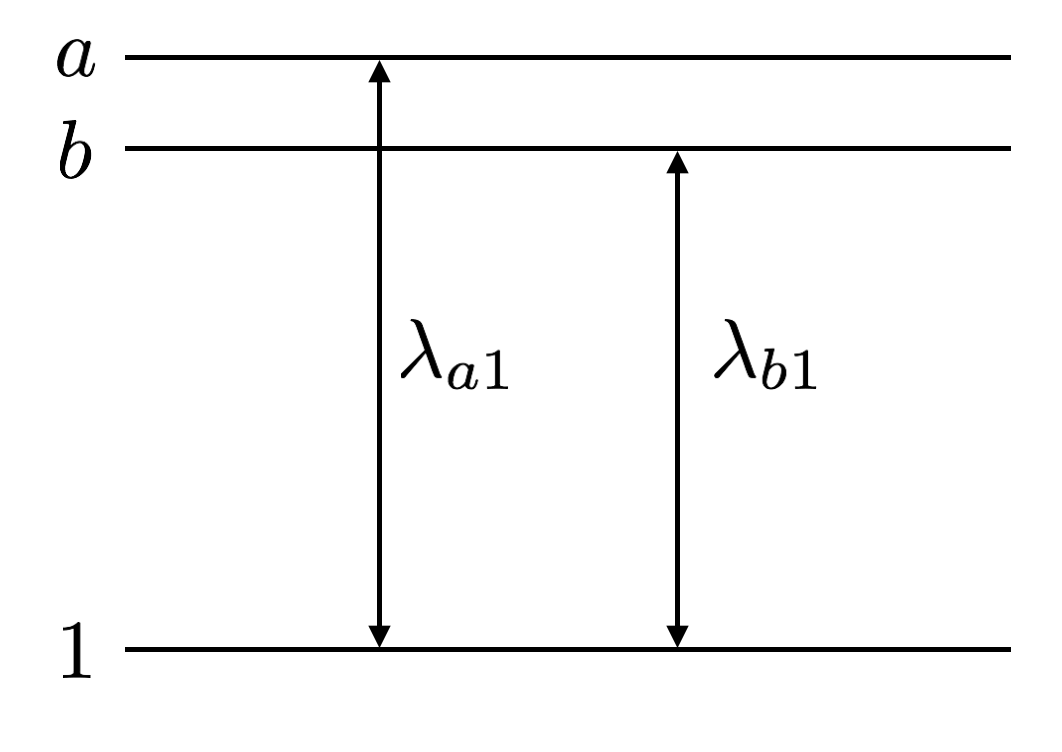
\includegraphics[width=8cm]{states.png}
\centering
\caption{}
\end{figure}

First we obtain the Einstein coefficients and their respective g-coefficients for the two $\mathrm{[O\,II]}$ forbidden lines:

\begin{figure}[h] \label{fig:table}
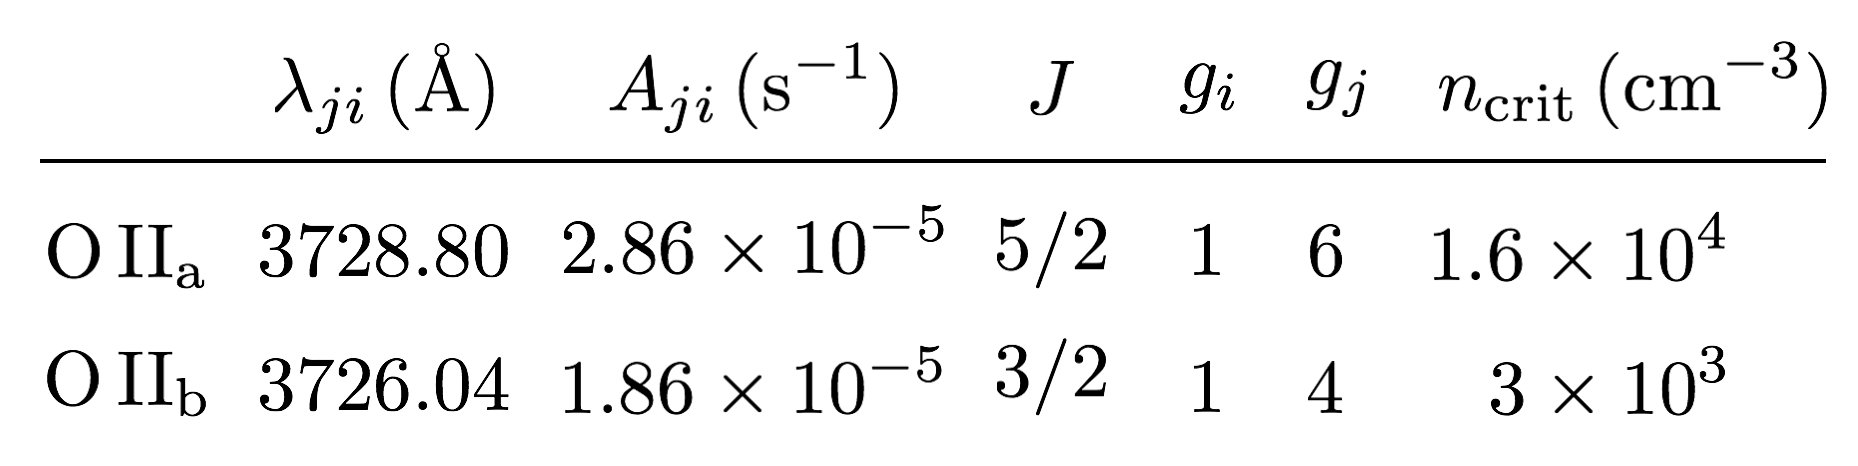
\includegraphics[width=8cm]{table.png}
\centering
\caption{}
\end{figure}

Before we derive the ratio of line fluxes $F_{a1}/F_{b1}$ for the two given scenarios, we can obtain its general form. For a line transitioning from state $j \rightarrow i$, the line flux $F_{ji}$ is determined by the number density of atoms in the upper state $n_j$, the volume of emitting gas $V$, the spontaneous emission Einstein coefficient $A_{ji}$,, the transition wavelength $\lambda_{ji}$, and the distance $r$ away:

\begin{align*}
F_{ji} = n_jVA_{ji}\left(\frac{hc}{\lambda_{ji}}\right) \left(\frac{1}{4\pi r^2}\right).
\end{align*}

Applying this to the $\mathrm{[O\,II]}$ transitions $a\rightarrow1$ and $b\rightarrow1$, we have

\begin{align*}
F_{a1} = n_aVA_{a1}\left(\frac{hc}{\lambda_{a1}}\right) \left(\frac{1}{4\pi r^2}\right)
\end{align*}

and

\begin{align*}
F_{b1} = n_bVA_{b1}\left(\frac{hc}{\lambda_{b1}}\right) \left(\frac{1}{4\pi r^2}\right).
\end{align*}

Taking their ratio, the emitting volume and distances cancel and we obtain:

\begin{align*}
\frac{F_{a1}}{F_{b1}} = \left(\frac{n_a}{n_b}\right) \left(\frac{A_{a1}}{A_{b1}}\right) \left(\frac{\lambda_{b1}}{\lambda_{a1}}\right).
\end{align*}

Since we know the Einstein coefficients and transition wavelengths, we need only find the number densities for each of the two scenarios.

\subsection*{Extremely low electron density}

With an extremely low electron density, we can assume that the forbidden lines are in non-LTE so we cannot use the Boltzmann distribution. However we can use the equation for statistical equilibrium which balances excitation with de-excitation. For the general case of transition between states $1 \leftarrow\rightarrow 2$:

\begin{align*}
n_1n_eq_{12} + n_1\bar{J}B_{12} = n_2n_eq_{12} + n_2B_{21}\bar{J} + n_2A_{21}
\end{align*}

where we recall that $A_{21}$, $B_{21}$ and $B_{12}$ are the Einstein coefficients for spontaneous emission, stimulated emission and stimulated absorption. Since we are in the optically thin regime, we can ignore $B_{12}$ and $B_{21}$:

\begin{align*}
n_1n_eq_{12} = n_2n_eq_{12} + n_2A_{21}.
\end{align*}

Solving for $n_2$:

\begin{align*}
n_1n_eq_{12} = n_2(n_eq_{12} + A_{21})
n_2 = \frac{n_1n_eq_{12}}{n_eq_{12} + A_{21}}.
\end{align*}

Recalling the definition of critical density for matter LTE, $n_\mathrm{crit} \equiv A/q$, the extremely low electron density regime that we're in suggests that:

\begin{align*}
n_e \ll n_\mathrm{crit}
n_e \ll \frac{A_{21}}{q_{21}}
n_eq_{a1} \ll A_{21}
\end{align*}

which allows us to simplify the denominator of $n_2$:

\begin{align*}
n_2 = \frac{n_1n_eq_{12}}{A_{21}}.
\end{align*}

Applying this to the number densities $n_a$ and $n_b$ for the $\mathrm{[O\,II]}$ transitions

\begin{align*}
n_a = \frac{n_1n_eq_{1a}}{A_{a1}}
n_b = \frac{n_1n_eq_{1b}}{A_{b1}}
\end{align*}

and taking their ratio:

\begin{equation*}
\begin{split}
\frac{n_a}{n_b} &= \frac{\left(\frac{n_1n_eq_{1a}}{A_{a1}}\right)}{\left(\frac{n_1n_eq_{1b}}{A_{b1}}\right)} \\
\frac{n_a}{n_b} &= \left(\frac{n_1n_eq_{1a}}{A_{a1}}\right) \left(\frac{A_{b1}}{n_1n_eq_{1b}}\right) \\
\frac{n_a}{n_b} &= \left(\frac{n_1n_eq_{1a}}{n_1n_eq_{1b}}\right) \left(\frac{A_{b1}}{A_{a1}}\right) \\
\frac{n_a}{n_b} &= \left(\frac{q_{1a}}{q_{1b}}\right) \left(\frac{A_{b1}}{A_{a1}}\right).
\end{split}
\end{equation*}

Substituting this into our general expression for the ratio of line fluxes and simplifying:

\begin{equation*}
\begin{split}
\frac{F_{a1}}{F_{b1}} &= \left(\frac{n_a}{n_b}\right) \left(\frac{A_{a1}}{A_{b1}}\right) \left(\frac{\lambda_{b1}}{\lambda_{a1}}\right). \\
\frac{F_{a1}}{F_{b1}} &= \left(\frac{q_{1a}}{q_{1b}}\frac{A_{b1}}{A_{a1}}\right) \left(\frac{A_{a1}}{A_{b1}}\right) \left(\frac{\lambda_{b1}}{\lambda_{a1}}\right). \\
\frac{F_{a1}}{F_{b1}} &= \left(\frac{q_{1a}}{q_{1b}}\right) \left(\frac{\lambda_{b1}}{\lambda_{a1}}\right).
\end{split}
\end{equation*}

We now need to find the excitation coefficients $q_{1a}$ and $q_{1b}$ which can be done using the relation for their ratio and the definition of critical density for matter LTE, $q \equiv A/n_\mathrm{crit}$:

\begin{equation*}
\begin{split}
\frac{q_{ij}}{q_{ji}} &= \left(\frac{g_j}{g_i}\right) \exp \left(\frac{- \Delta E_{ji}}{k_BT}\right) \\
q_{ij} &= q_{ji} \left(\frac{g_j}{g_i}\right) \exp \left(\frac{- \Delta E_{ji}}{k_BT}\right) \\
q_{ij} &= \left(\frac{A_{ji}}{n_\mathrm{crit}}\right) \left(\frac{g_j}{g_i}\right) \exp \left(\frac{- \Delta E_{ji}}{k_BT}\right).
\end{split}
\end{equation*}

Applying this to the $\mathrm{[O\,II]}$ transitions:

\begin{equation*}
\begin{split}
q_{1a} &= \left(\frac{A_{a1}}{n_\mathrm{crit,a1}}\right) \left(\frac{g_a}{g_1}\right) \exp \left(\frac{- \Delta E_{a1}}{k_BT}\right) \\
q_{1a} &= \left(\frac{A_{a1}}{n_\mathrm{crit,a1}}\right) \left(\frac{g_a}{g_1}\right) \exp \left(\frac{- (hc/\lambda_{a1})}{k_BT}\right) \\
q_{1a} &= \left(\frac{A_{a1}}{n_\mathrm{crit,a1}}\right) \left(\frac{g_a}{g_1}\right) \exp \left(\frac{- hc}{k_BT\lambda_{a1}}\right)
\end{split}
\end{equation*}

and

\begin{equation*}
\begin{split}
q_{1b} &= \left(\frac{A_{b1}}{n_\mathrm{crit,b1}}\right) \left(\frac{g_b}{g_1}\right) \exp \left(\frac{- \Delta E_{b1}}{k_BT}\right) \\
q_{1b} &= \left(\frac{A_{b1}}{n_\mathrm{crit,b1}}\right) \left(\frac{g_b}{g_1}\right) \exp \left(\frac{- (hc/\lambda_{b1})}{k_BT}\right) \\
q_{1b} &= \left(\frac{A_{b1}}{n_\mathrm{crit,b1}}\right) \left(\frac{g_b}{g_1}\right) \exp \left(\frac{- hc}{k_BT\lambda_{b1}}\right).
\end{split}
\end{equation*}

Returning to our expression for the line flux ratio and plugging in $q_{1a}$ and $q_{1b}$, we obtain the solution for an extremely low electron density:

\begin{equation*}
\begin{split}
\frac{F_{a1}}{F_{b1}} &= \left(\frac{q_{1a}}{q_{1b}}\right) \left(\frac{\lambda_{b1}}{\lambda_{a1}}\right) \\
\frac{F_{a1}}{F_{b1}} &= \left(\frac{\left(\frac{A_{a1}}{n_\mathrm{crit,a1}}\right) \left(\frac{g_a}{g_1}\right) \exp \left(\frac{- hc}{k_BT\lambda_{a1}}\right)}{\left(\frac{A_{b1}}{n_\mathrm{crit,b1}}\right) \left(\frac{g_b}{g_1}\right) \exp \left(\frac{- hc}{k_BT\lambda_{b1}}\right)}\right) \left(\frac{\lambda_{b1}}{\lambda_{a1}}\right) \\
\frac{F_{a1}}{F_{b1}} &= \left(\frac{A_{a1}}{n_\mathrm{crit,a1}}\right) \left(\frac{g_a}{g_1}\right) \exp \left(\frac{- hc}{k_BT\lambda_{a1}}\right) \cdot \left(\frac{n_\mathrm{crit,b1}}{A_{b1}}\right) \left(\frac{g_1}{g_b}\right) \exp \left(\frac{hc}{k_BT\lambda_{b1}}\right) \left(\frac{\lambda_{b1}}{\lambda_{a1}}\right) \\
\frac{F_{a1}}{F_{b1}} &= \left(\frac{A_{a1}}{A_{b1}}\right) \left(\frac{g_a}{g_b}\right) \left(\frac{n_\mathrm{crit,b1}}{n_\mathrm{crit,a1}}\right) \exp \left(\frac{- hc}{k_BT\lambda_{a1}}\right) \exp \left(\frac{hc}{k_BT\lambda_{b1}}\right) \left(\frac{\lambda_{b1}}{\lambda_{a1}}\right) \\
\frac{F_{a1}}{F_{b1}} &= \left(\frac{A_{a1}}{A_{b1}}\right) \left(\frac{g_a}{g_b}\right) \left(\frac{n_\mathrm{crit,b1}}{n_\mathrm{crit,a1}}\right) \left(\frac{\lambda_{b1}}{\lambda_{a1}}\right) \exp \left(\frac{- hc}{k_BT\lambda_{a1}} + \frac{hc}{k_BT\lambda_{b1}}\right) \\
\frac{F_{a1}}{F_{b1}} &= \left(\frac{A_{a1}}{A_{b1}}\right) \left(\frac{g_a}{g_b}\right) \left(\frac{n_\mathrm{crit,b1}}{n_\mathrm{crit,a1}}\right) \left(\frac{\lambda_{b1}}{\lambda_{a1}}\right) \exp \left(\frac{hc}{k_BT} \left(\frac{1}{\lambda_{b1}} - \frac{1}{\lambda_{a1}}\right)\right).
\end{split}
\end{equation*}

Plugging in values,

\begin{equation*}
\begin{split}
\frac{F_{a1}}{F_{b1}} &= \left(\frac{2.86\times10^{-5}}{1.86\times10^{-5}}\right) \left(\frac{6}{4}\right) \left(\frac{3\times10^3\,\mathrm{cm^{-3}}}{1.6\times10^4\,\mathrm{cm^{-3}}}\right) \left(\frac{3726.04\,\mathrm{A}}{3728.8\,\mathrm{A}}\right) \exp \left(\frac{hc}{k_B(10^4\,\mathrm{K})} \left(\frac{1}{3726.04\,\mathrm{A}} - \frac{1}{3728.8\,\mathrm{A}}\right)\right)
\end{split}
\end{equation*}

\begin{align*}
\boxed{ \frac{F_{a1}}{F_{b1}} = 0.43 }.
\end{align*}

\subsection*{Extremely high electron density}

Recall that we need to find the number densities of each energy level to complete our solution from the generic case. For an extremely high electron density, we can assume that both line transitions are in LTE which allows us to use the Boltzmann equation for the relative population of number densities with respect to the ground state:

\begin{equation*}
\begin{split}
\frac{n_a}{n_1} &= \left(\frac{g_a}{g_1}\right) \exp \left(\frac{- \Delta E_{a1}}{k_BT}\right) \\
\frac{n_a}{n_1} &= \left(\frac{g_a}{g_1}\right) \exp \left(\frac{- (hc/\lambda_{a1})}{k_BT}\right) \\
\frac{n_a}{n_1} &= \left(\frac{g_a}{g_1}\right) \exp \left(\frac{-hc}{k_BT\lambda_{a1}}\right)
\end{split}
\end{equation*}

and

\begin{equation*}
\begin{split}
\frac{n_b}{n_1} &= \left(\frac{g_b}{g_1}\right) \exp \left(\frac{- \Delta E_{b1}}{k_BT}\right) \\
\frac{n_b}{n_1} &= \left(\frac{g_b}{g_1}\right) \exp \left(\frac{- (hc/\lambda_{b1})}{k_BT}\right) \\
\frac{n_b}{n_1} &= \left(\frac{g_b}{g_1}\right) \exp \left(\frac{-hc}{k_BT\lambda_{b1}}\right).
\end{split}
\end{equation*}

Taking their ratios:

\begin{equation*}
\begin{split}
\frac{\left(\frac{n_a}{n_1}\right)}{\left(\frac{n_b}{n_1}\right)} &= \frac{\left(\frac{g_a}{g_1}\right) \exp \left(\frac{-hc}{k_BT\lambda_{a1}}\right)}{\left(\frac{g_b}{g_1}\right) \exp \left(\frac{-hc}{k_BT\lambda_{b1}}\right)} \\
\frac{n_a}{n_1} \cdot \frac{n_1}{n_b} &= \left(\frac{g_a}{g_1}\right) \exp \left(\frac{-hc}{k_BT\lambda_{a1}}\right) \cdot \left(\frac{g_1}{g_b}\right) \exp \left(\frac{hc}{k_BT\lambda_{b1}}\right) \\
\frac{n_a}{n_b} &= \left(\frac{g_a}{g_b}\right) \exp \left(\frac{-hc}{k_BT\lambda_{a1}} + \frac{hc}{k_BT\lambda_{b1}} \right) \\
\frac{n_a}{n_b} &= \left(\frac{g_a}{g_b}\right) \exp \left(\frac{hc}{k_BT\lambda_{a1}} \left(\frac{1}{\lambda_{b1}} - \frac{1}{\lambda_{a1}}\right) \right).
\end{split}
\end{equation*}

Substituting this into our general equation for the ratio of line fluxes, we obtain the solution for an extremely high electron density:

\begin{equation*}
\begin{split}
\frac{F_{a1}}{F_{b1}} &= \left(\frac{n_a}{n_b}\right) \left(\frac{A_{a1}}{A_{b1}}\right) \left(\frac{\lambda_{b1}}{\lambda_{a1}}\right) \\
\frac{F_{a1}}{F_{b1}} &= \left(\frac{A_{a1}}{A_{b1}}\right) \left(\frac{g_a}{g_b}\right) \left(\frac{\lambda_{b1}}{\lambda_{a1}}\right) \exp \left(\frac{hc}{k_BT\lambda_{a1}} \left(\frac{1}{\lambda_{b1}} - \frac{1}{\lambda_{a1}}\right) \right). 
\end{split}
\end{equation*}

Plugging in values,

\begin{equation*}
\begin{split}
\frac{F_{a1}}{F_{b1}} &= \left(\frac{2.86\times10^{-5}}{1.86\times10^{-5}}\right) \left(\frac{6}{4}\right) \left(\frac{3726.04\,\mathrm{A}}{3728.8\,\mathrm{A}}\right) \exp \left(\frac{hc}{k_B(10^4\,\mathrm{K})} \left(\frac{1}{3726.04\,\mathrm{A}} - \frac{1}{3728.8\,\mathrm{A}}\right)\right)
\end{split}
\end{equation*}

\begin{align*}
\boxed{ \frac{F_{a1}}{F_{b1}} = 2.31 }.
\end{align*}

% --------------------------------------------------------------
%               Part 2)
% --------------------------------------------------------------

\subsection*{Part 2}

How does the flux ratio vary when the density varies from, say, $1\,\mathrm{cm^{-3}}$ to $10^5\mathrm{cm^{-3}}$? How does your result depend on the temperature of the $\mathrm{HII}$ region?

% --------------------------------------------------------------
%               Solution
% --------------------------------------------------------------

\subsection*{Solution}

With an electron density of $1\,\mathrm{cm^{-3}}$, we are in the non-LTE regime since $n_e \ll n_\mathrm{crit,a1}$ and $n_e \ll n_\mathrm{crit,b1}$. We can therefore use the expression for the ratio of line fluxes derived in part 1 for non-LTE (i.e., extremely low electron density):

\begin{align*}
\frac{F_{a1}}{F_{b1}} = \left(\frac{A_{a1}}{A_{b1}}\right) \left(\frac{g_a}{g_b}\right) \left(\frac{n_\mathrm{crit,b1}}{n_\mathrm{crit,a1}}\right) \exp \left(\frac{hc}{k_BT} \left(\frac{1}{\lambda_{b1}} - \frac{1}{\lambda_{a1}}\right)\right)
\end{align*}

\begin{align*}
\boxed{ \frac{F_{a1}}{F_{b1}} = 0.43 }.
\end{align*}

Conversely, with an electron density of $10^5\,\mathrm{cm^{-3}}$, we are in the LTE regime since $n_e \gg n_\mathrm{crit,a1}$ and $n_e \gg n_\mathrm{crit,b1}$. We can therefore use the expression for the ratio of line fluxes derived in part 1 for LTE (i.e., extremely high electron density):

\begin{align*}
\frac{F_{a1}}{F_{b1}} = \left(\frac{A_{a1}}{A_{b1}}\right) \left(\frac{g_a}{g_b}\right) \left(\frac{\lambda_{b1}}{\lambda_{a1}}\right) \exp \left(\frac{hc}{k_BT\lambda_{a1}} \left(\frac{1}{\lambda_{b1}} - \frac{1}{\lambda_{a1}}\right) \right).
\end{align*}

\begin{align*}
\boxed{ \frac{F_{a1}}{F_{b1}} = 2.31 }.
\end{align*}

Therefore the line flux ratio varies from 0.4 to 2.3 when the density varies from $1\,\mathrm{cm^{-3}}$ (NLTE) to $10^5\,\mathrm{cm^{-3}}$ (LTE).

% --------------------------------------------------------------
%                    4. 
% --------------------------------------------------------------

\section{Spectral Energy Distribution of a Protoplanetary Disk}

We produce a theoretical prediction for the spectral energy distribution (SED) of a minimum-mass-solar nebula (one that is needed to account for all planet masses) around a sun-like star. The (gas+dust) surface mass density (measured perpendicular to the disk plane) of such a disk goes with radius as $\Sigma = 1700(r/\mathrm{AU})^{-3/2}\,\mathrm{g/cm^2}$, out of which 1\% is dust. Dust grains have a size distribution of $dN/ds = c(r)s^{-3.5}$ everywhere, with a minimum size of $s_\mathrm{min}$ and a maximum size of $s_\mathrm{max}$. You can assume $s_\mathrm{min} \sim 0.01\,\mu\mathrm{m}$ and $s_\mathrm{max}$ is sitting somewhere between $100\,\mu\mathrm{m}$ and $100\,\mathrm{km}$.

% --------------------------------------------------------------
%               Part 1)
% --------------------------------------------------------------

\subsection*{Part 1}

Consider the mass opacity ($\kappa_\nu = n\sigma_\nu/\rho$) in the disk. Derive its dependence on $s_\mathrm{max}$ and $\nu$ for the two limits: $s_\mathrm{max} \gg \lambda$ and $s_\mathrm{max} \ll \lambda $. (\textit{Hint: For the former case you have to consider opacity in the $s_\mathrm{max} \gg \lambda$ and $s_\mathrm{max} \ll \lambda$ ranges separately. $\lambda$ is the photon wavelength.})

% --------------------------------------------------------------
%               Solution
% --------------------------------------------------------------

\subsection*{Solution}

Starting with the definition of mass opacity

\begin{align*}
\kappa_\nu = \frac{n \sigma_\nu}{\rho_\mathrm{disk}}
\end{align*}

and re-writing the mass density of the disk in terms of the dust grains:

\begin{equation*}
\begin{split}
\kappa_\nu &= \frac{n \sigma_\nu}{\frac{4}{3}\pi s^3 n\rho_\mathrm{dust}} \\
\kappa_\nu &= \frac{\sigma_\nu}{\frac{4}{3}\pi s^3 \rho_\mathrm{dust}}.
\end{split}
\end{equation*}

The extinction cross section $\sigma_\mathrm{ext}$ can be used which is a combination of scattering and absorption:
 
\begin{align*}
\sigma_\mathrm{ext} = \sigma_\mathrm{abs} + \sigma_\mathrm{scat}.
\end{align*}

The extinction cross section $\sigma_\mathrm{ext}$ is given by the following for small grains

\begin{equation*}
\begin{split}
\sigma_\mathrm{ext}(s<\lambda) \approx \pi s^2 \left(\left(\frac{s}{\lambda}\right) + \left(\frac{s}{\lambda}\right)\right) = \pi s^2 \left(\left(\frac{s\nu}{c}\right) + \left(\frac{s\nu}{c}\right)^4\right)
\end{split}
\end{equation*}

which is simplified for large grains to

\begin{align*}
\sigma_\mathrm{ext}(s>\lambda) \approx \pi s^2.
\end{align*}

Applying this to the mass opacity for a given dust grain size $s$ and observing wavelength $\lambda$, 

\begin{equation*}
\begin{split}
\kappa_\nu(s<\lambda) &\approx \frac{\pi s^2 \left(\left(\frac{s\nu}{c}\right) + \left(\frac{s\nu}{c}\right)^4\right)}{\frac{4}{3}\pi s^3 \rho_\mathrm{dust}} \\
\kappa_\nu(s<\lambda) &\approx \frac{3\left(\left(\frac{s\nu}{c}\right) + \left(\frac{s\nu}{c}\right)^4\right)}{4s \rho_\mathrm{dust}}
\end{split}
\end{equation*}

and 

\begin{equation*}
\begin{split}
\kappa_\nu(s>\lambda) &\approx \frac{\pi s^2}{\frac{4}{3}\pi s^3 \rho_\mathrm{dust}} \\
\kappa_\nu(s>\lambda) &\approx \frac{3}{4s\rho_\mathrm{dust}}.
\end{split}
\end{equation*}

To get the total mass opacity, $\kappa_\nu$ needs to be integrated over all dust grain sizes $s$:

\begin{equation*}
\begin{split}
\kappa_\nu &= \int\kappa_\nu(s<\lambda)\frac{dN}{ds}ds + \int\kappa_\nu(s>\lambda)\frac{dN}{ds}ds \\
\kappa_\nu &= \int \frac{3\left(\left(\frac{s\nu}{c}\right) + \left(\frac{s\nu}{c}\right)^4\right)}{4s \rho_\mathrm{dust}} \frac{dN}{ds}ds + \int \pi s^2 \frac{dN}{ds}ds
\end{split}
\end{equation*}

Making the substitution

\begin{align*}
\frac{dN}{ds} = c(r)s^{-3.5}
\end{align*}

for the dust grain size distribution, we get the following general expression for the mass opacity:

\begin{equation*}
\begin{split}
\kappa_\nu = \int_{s_\mathrm{min}}^\lambda \frac{3\left(\left(\frac{s\nu}{c}\right) + \left(\frac{s\nu}{c}\right)^4\right)}{4s \rho_\mathrm{dust}} c(r)s^{-3.5}ds + \int_\lambda^{s_\mathrm{max}} \frac{3}{4s\rho_\mathrm{dust}} c(r)s^{-3.5}ds
\end{split}
\end{equation*}

where the integration limits reflect the fact that small grains have sizes $s_\mathrm{min}<s<\lambda$ and large grains have sizes $\lambda<s<s_\mathrm{max}$.

Following through with integration:

\begin{equation*}
\begin{split}
\kappa_\nu &= \frac{3c(r)}{4\rho_\mathrm{dust}} \int_{s_\mathrm{min}}^\lambda \frac{\left(\left(\frac{s\nu}{c}\right) + \left(\frac{s\nu}{c}\right)^4\right)}{s} s^{-3.5}ds + \frac{3c(r)}{4\rho_\mathrm{dust}} \int_\lambda^{s_\mathrm{max}} \frac{1}{s}s^{-3.5}ds \\
\kappa_\nu &= \frac{3c(r)}{4\rho_\mathrm{dust}} \int_{s_\mathrm{min}}^\lambda \frac{1}{s}\left(\left(\frac{s\nu}{c}\right) + \left(\frac{s\nu}{c}\right)^4\right) s^{-3.5}ds + \frac{3c(r)}{4\rho_\mathrm{dust}} \int_\lambda^{s_\mathrm{max}} s^{-1}s^{-3.5}ds \\
\kappa_\nu &= \frac{3c(r)}{4\rho_\mathrm{dust}} \int_{s_\mathrm{min}}^\lambda \left(\left(\frac{s\nu}{c}\right)\frac{s^{-3.5}}{s} + \left(\frac{s\nu}{c}\right)^4\frac{s^{-3.5}}{s}\right)ds + \frac{3c(r)}{4\rho_\mathrm{dust}} \int_\lambda^{s_\mathrm{max}} s^{-4.5}ds \\
\kappa_\nu &= \frac{3c(r)}{4\rho_\mathrm{dust}} \int_{s_\mathrm{min}}^\lambda \left(\left(\frac{\nu}{c}\right)s\frac{s^{-3.5}}{s} + \left(\frac{\nu}{c}\right)^4s^4\frac{s^{-3.5}}{s}\right)ds + \frac{3c(r)}{4\rho_\mathrm{dust}} \int_\lambda^{s_\mathrm{max}} s^{-4.5}ds \\
\kappa_\nu &= \frac{3c(r)}{4\rho_\mathrm{dust}} \int_{s_\mathrm{min}}^\lambda \left(\left(\frac{\nu}{c}\right)s^{-3.5} + \left(\frac{\nu}{c}\right)^4s^{-0.5}\right)ds + \frac{3c(r)}{4\rho_\mathrm{dust}} \int_\lambda^{s_\mathrm{max}} s^{-4.5}ds \\
\kappa_\nu &= \frac{3c(r)}{4\rho_\mathrm{dust}} \left\{\left(\frac{\nu}{c}\right)\int_{s_\mathrm{min}}^\lambda s^{-3.5}ds + \left(\frac{\nu}{c}\right)^4 \int_{s_\mathrm{min}}^\lambda s^{-0.5}ds\right\} + \frac{3c(r)}{4\rho_\mathrm{dust}} \int_\lambda^{s_\mathrm{max}} s^{-4.5}ds \\
\kappa_\nu &= \frac{3c(r)}{4\rho_\mathrm{dust}} \left\{\left(\frac{\nu}{c}\right) \left[\frac{s^{-2.5}}{-2.5}\right]_{s_\mathrm{min}}^\lambda + \left(\frac{\nu}{c}\right)^4 \left[\frac{s^{0.5}}{0.5}\right]_{s_\mathrm{min}}^\lambda \right\} + \frac{3c(r)}{4\rho_\mathrm{dust}} \left[\frac{s^{-3.5}}{-3.5}\right]_\lambda^{s_\mathrm{max}} \\
\kappa_\nu &= \frac{3c(r)}{4\rho_\mathrm{dust}} \left\{\left(\frac{\nu}{c}\right) \left[\frac{s^{-2.5}}{2.5}\right]^{s_\mathrm{min}}_\lambda + \left(\frac{\nu}{c}\right)^4 \left[\frac{s^{0.5}}{0.5}\right]_{s_\mathrm{min}}^\lambda + \left[\frac{s^{-3.5}}{3.5}\right]^\lambda_{s_\mathrm{max}} \right\} \\
\kappa_\nu &= \frac{3c(r)}{4\rho_\mathrm{dust}} \left\{\frac{1}{2.5}\left(\frac{\nu}{c}\right) \left[s_\mathrm{min}^{-2.5} - \lambda^{-2.5}\right] + \frac{1}{0.5}\left(\frac{\nu}{c}\right)^4 \left[\lambda^{0.5} - s_\mathrm{min}^{0.5}\right] + \frac{1}{3.5}\left[\lambda^{-3.5} - s_\mathrm{max}^{-3.5}\right] \right\} \\
\kappa_\nu &= \frac{3c(r)}{4\rho_\mathrm{dust}} \left\{\frac{2}{5}\left(\frac{\nu}{c}\right) \left[s_\mathrm{min}^{-5/2} - \lambda^{-5/2}\right] + 2\left(\frac{\nu}{c}\right)^4 \left[\lambda^{1/2} - s_\mathrm{min}^{1/2}\right] + \frac{2}{7}\left[\lambda^{-7/2} - s_\mathrm{max}^{-7/2}\right] \right\}.
\end{split}
\end{equation*}

Therefore, in the limit that $s_\mathrm{max}\gg\lambda$, the mass opacity scales as $\kappa_\nu \propto s_\mathrm{max}^{-7/2}$ and in the limit that $s_\mathrm{max}\ll\lambda$, the mass opacity scales as $\kappa_\nu \propto s_\mathrm{max}^{-5/2}$.

% --------------------------------------------------------------
%               Part 2)
% --------------------------------------------------------------

\subsection*{Part 2}

Outside of what radius is the disk optically thin (vertically) to optical light, and thin to submm (say, $0.1\,\mathrm{cm}$) radiation, respectively? Typical disks have sizes $<1000\,\mathrm{AU}$.

% --------------------------------------------------------------
%               Solution
% --------------------------------------------------------------

\subsection*{Solution}



% --------------------------------------------------------------
%               Part 3)
% --------------------------------------------------------------

\subsection*{Part 3}

Write down the thermal emission from a ring at radius $r$ in the optically thick limit. Integrate over the disk ($r_\mathrm{mim}$ to $r_\mathrm{max}$) to obtain the frequency slope of the integrated flux $F_\nu$ at the submm wavelength. Are you in the Rayleigh-Jeans tail? Do your results depend on dust mass and/or dust sizes? For disk temperature, assume a simple law of $T\propto250\,\mathrm{K}(r/\mathrm{AU})^{-1/2}$, independent of grain size.

% --------------------------------------------------------------
%               Solution
% --------------------------------------------------------------

\subsection*{Solution}

In the optically thick limit, the thermal emission is that of a blackbody at temperature $T$:

\begin{align*}
I_\nu = B_\nu(T) = \frac{2h\nu}{c^2} \frac{1}{\exp(h\nu/k_BT) -1}.
\end{align*}

Assuming temperature scales with radius as $T \propto 250\,\mathrm{K}(r/\mathrm{AU})^{-1/2}$,

\begin{align*}
I_\nu = B_\nu(T) = \frac{2h\nu}{c^2} \frac{1}{\exp\left(\frac{h\nu}{250k_BT}\sqrt{\frac{r}{\mathrm{AU}}}\right) -1}.
\end{align*}

% --------------------------------------------------------------
%               Part 4)
% --------------------------------------------------------------

\subsection*{Part 4}

Now repeat the exercise in the optically thin limit. Obtain the slope of the integrated spectrum, $F_\nu$, as well as any dependence on $s_\mathrm{max}$. (\textit{Hint: When you integrate the flux over radius, be sure to include the radius dependence of $c(r)$. Also, differentiate between the case where $s_\mathrm{max} \gg \lambda$ and $s_\mathrm{min} \ll \lambda$.})

% --------------------------------------------------------------
%               Solution
% --------------------------------------------------------------

\subsection*{Solution}



% --------------------------------------------------------------
%               Part 5)
% --------------------------------------------------------------

\subsection*{Part 5}

Grains in the disk can grow by conglomeration. What happens to the SED when $s_\mathrm{max}$ increases from $100\,\mu\mathrm{m}$ to $100\,\mathrm{km}$?

Now you are ready to observe (as Andrews \& Williams 2007 did).

% --------------------------------------------------------------
%               Solution
% --------------------------------------------------------------

\subsection*{Solution}





\end{document}
